\subsection{Сбор набора данных}
Сбор качественного и репрезентативного набора данных является ключевым этапом при реализации задач генеративного компьютерного зрения, в частности "--- виртуальной примерочной одежды. От полноты и разнообразия исходных данных напрямую зависит успешность обучения моделей и достоверность последующих экспериментов.

Одной из главных задач практической части работы является сбор собственного набора данных. Это необходимо для независимости проводимых экспериментов. Был собран набор данных из 110 изображений людей в различных позах, а также парные к ним 110 изображений верхней одежды. В дальнейшем, с помощью скриптов и специализированных нейронных сетей, удалось получить необходимые дополнительные данные для набора. В частности:
\begin{itemize}
    \item \texttt{openpose\_img}, \texttt{openpose\_json} "--- выходы модели \texttt{OpenPose}, предназначенной для получения информации о позе человека на фотографии. Пример фотографии из \texttt{openpose\_img} можно увидеть на изображении \ref{fig:practice_openpose} \cite{8765346}. \texttt{openpose\_json} для каждой фотографии содержит отдельный \texttt{.json} файл, содержащий координаты ключевой точки, а также уверенность модели в том, что эта ключевая точка действительно должна быть по этим координатам. К ключевой точке можно отнести части тела, выделяющие позу человека. Например, левое плечо, правой плечо, шея, таз. Эти маски необходимы для корректного наложения новой одежды на изображения, чтобы учитывать позу и общее положение исходной одежды \cite{8765346};
    \item \texttt{cloth\_mask} представляет собой набор бинарных масок, где белый пиксель соответствует одежде, а чёрный "--- всему остальному. Эта маска необходима для корректной работы моделей сегментации;
    \item \texttt{agnostic\_mask} является набором бинарных масок одежды, полученные в результате парсинга одежды с исходного изображения модели. Необходима для того, чтобы учитывать, в каком положении находилась исходная одежда;
    \item \texttt{test\_pairs.txt} "--- текстовый файл, каждая строка которого содержит пару имён изображений. Это необходимо для моделей, работающих с парными изображениями. Первое имя является изображением, из которого берётся одежда, второе имя является результирующим изображением, на котором эта одежда будет изображена;
    \item \texttt{test\_gpt4o.json} содержит в себе текстовые описания позы и человека, необходимые для \texttt{PromptDresser}.
\end{itemize}

Ниже представлена общая структура собранного набора данных:
\begin{verbatim}
course_dataset/
    |--image/
    |--cloth/
    |--agnostic-mask/
    |--cloth-mask/
    |--image-densepose/
    |--image-parse-v3/
    |--openpose_img/
    |--openpose_json/
    |--test_gpt4o.json
    |--test_pairs.txt
\end{verbatim}

\begin{figure}[H]
    \centering
    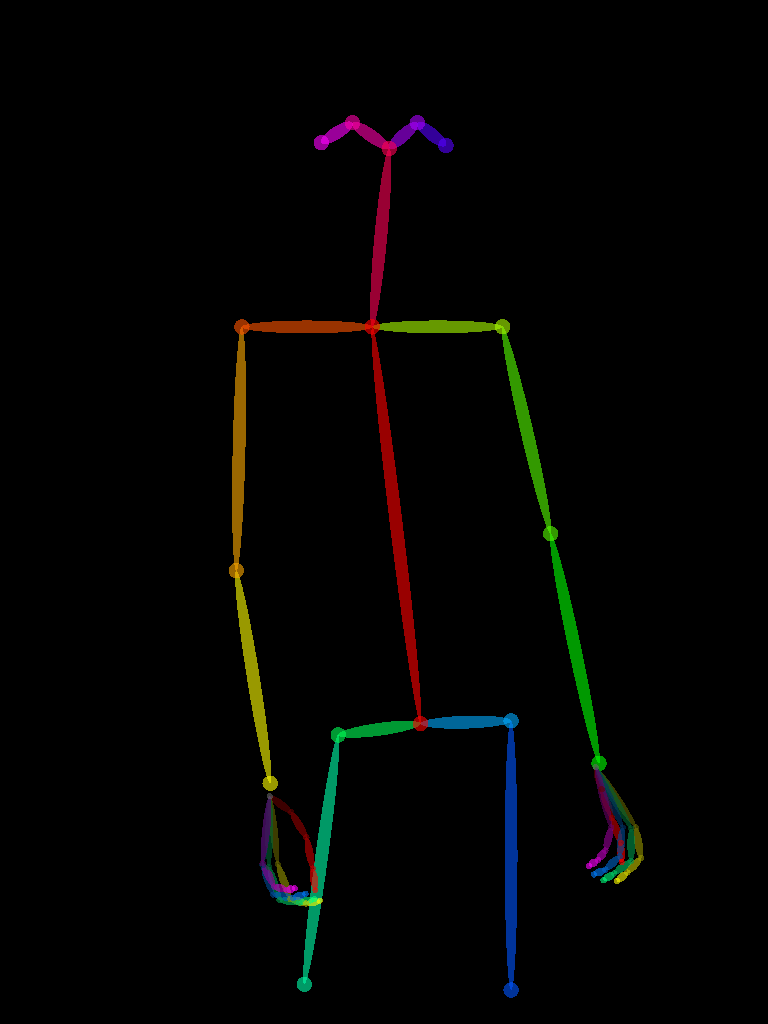
\includegraphics[width=0.55\linewidth]{images/practice_openpose.png}
    \caption{Пример изображения из \texttt{openpose\_img}}
    \label{fig:practice_openpose}
\end{figure}
